\documentclass[conference]{IEEEtran}
\ifCLASSINFOpdf

\else

\fi
\usepackage{graphicx}
\hyphenation{op-tical net-works semi-conduc-tor}


\begin{document}
%
% paper title
% can use linebreaks \\ within to get better formatting as desired
% Do not put math or special symbols in the title.
\title{Linearization of Capacitive Level Sensor using Soft Computing Techniques}


% author names and affiliations
% use a multiple column layout for up to three different
% affiliations
\author{\IEEEauthorblockN{Srikanth Malla}
\IEEEauthorblockA{B.Tech, VIT University,\\ Vellore, 632014,\\ India\\
Email: malla.srikanth2012@vit.ac.in}
\and
\IEEEauthorblockN{Venkata Lakshmi Narayana.K}
\IEEEauthorblockA{ Program Chair, SELECT,\\ VIT University,\\ Vellore, 632014,\\ India\\
Email: kvlnarayana@vit.ac.in}}
% \and
% \IEEEauthorblockN{James Kirk\\ and Montgomery Scott}
% \IEEEauthorblockA{Starfleet Academy\\
% San Francisco, California 96678-2391\\
% Telephone: (800) 555--1212\\
% Fax: (888) 555--1212}}

% conference papers do not typically use \thanks and this command
% is locked out in conference mode. If really needed, such as for
% the acknowledgment of grants, issue a \IEEEoverridecommandlockouts
% after \documentclass

% for over three affiliations, or if they all won't fit within the width
% of the page, use this alternative format:
% 
%\author{\IEEEauthorblockN{Michael Shell\IEEEauthorrefmark{1},
%Homer Simpson\IEEEauthorrefmark{2},
%James Kirk\IEEEauthorrefmark{3}, 
%Montgomery Scott\IEEEauthorrefmark{3} and
%Eldon Tyrell\IEEEauthorrefmark{4}}
%\IEEEauthorblockA{\IEEEauthorrefmark{1}School of Electrical and Computer Engineering\\
%Georgia Institute of Technology,
%Atlanta, Georgia 30332--0250\\ Email: see http://www.michaelshell.org/contact.html}
%\IEEEauthorblockA{\IEEEauthorrefmark{2}Twentieth Century Fox, Springfield, USA\\
%Email: homer@thesimpsons.com}
%\IEEEauthorblockA{\IEEEauthorrefmark{3}Starfleet Academy, San Francisco, California 96678-2391\\
%Telephone: (800) 555--1212, Fax: (888) 555--1212}
%\IEEEauthorblockA{\IEEEauthorrefmark{4}Tyrell Inc., 123 Replicant Street, Los Angeles, California 90210--4321}}




% use for special paper notices
%\IEEEspecialpapernotice{(Invited Paper)}




% make the title area
\maketitle

% As a general rule, do not put math, special symbols or citations
% in the abstract
\begin{abstract}
The  capacitive  level  sensors  are  most  commonly  used  sensors  for  the  measurement  of  liquid level in  the  industries. It  is  because  of  their  high  sensitivity,  less  power  dissipation  and ruggedness in design. However, in a capacitance sensor, the problem of high nonlinear response characteristics as well as dependence on the permittivity of liquid have imposed some restriction on the optimal use of such sensors. This paper compares different soft-computing algorithms and their performances. 

\end{abstract}

% no keywords




% For peer review papers, you can put extra information on the cover
% page as needed:
% \ifCLASSOPTIONpeerreview
% \begin{center} \bfseries EDICS Category: 3-BBND \end{center}
% \fi
%
% For peerreview papers, this IEEEtran command inserts a page break and
% creates the second title. It will be ignored for other modes.
\IEEEpeerreviewmaketitle



\section{Introduction}
% no \IEEEPARstart
There can be many direct and indirect methods for increasing the linearity of sensor response. ANN applies one such method. The advantages of using ANN for increasing the linearity range are ease of programming and software portability. It uses the synaptic weights for the training to minimize the error between the desired output and the actual output. After training the hardwired version of neural network (with fixed synaptic weights) can be cascaded with the sensor in order to cancel the sensor’s nonlinear characteristics. [1]\\
Jagdish Chandra Patra et al. propose Neural networks based scheme, when there is a change in ambient temperature, the ANN automatically compensates for this change based on the learning which it undergoes and on the information stored in its weights. The effect of change in environmental conditions on the capacitive sensors and subsequently upon the output is nonlinear in nature. Especially, change in ambient temperature causes response characteristics of the sensor to become highly nonlinear, and complex signal processing may be required to obtain correct readout. The purpose of direct modeling is to obtain an ANN model of the sensor in such a way that the outputs of the sensor and the ANN match closely. ANN model has been found to be capable of accurately estimating at any ambient temperature from $20^o$C to $70^o$C. This fact is the novel characteristic of the proposed ANN model. [2]\\
Artificial neural networks have emerged as a powerful learning technique to perform complex tasks nonlinear dynamic environments. An intelligent pressure sensor based on artificial neural networks to realize auto-calibration and nonlinear compensation of a CPS has been proposed with quite satisfactory performance. This technique can also be applied for other parameters such level etc. There are also some drawbacks of neural networks, such as neural networks can’t tell the redundant information from a huge amount of data, which will easily lead to some problems such as long training time and much computation. [3]\\
As explained in the paper [4], the nonlinear operation of a Multi layer perceptron (MLP) neural network compensates the nonlinear characteristics of a sensor. Sensor linearization can be considered a function estimation (modeling) task, where the non-linear sensor output can be used as input data and the desired linearized response as target data. 
The capability of a trained network can be measured to some extent by the errors on the training, validation and test sets. This can be done by applying unseen input to network and trace the output and compare with the sensor output. It has been proved successful in representing any measurable function within any desired degree of accuracy, with the correct values of pressures and sufficient number of hidden neurons. [5]
% % You must have at least 2 lines in the paragraph with the drop letter
% % (should never be an issue)
% I wish you the best of success.

% \hfill mds
 
% \hfill December 27, 2012

\subsection{Hardware Description}
Switzer manufacturer’s capacitive level transmitter is used for the experimentation, whose specifications are shown in the table1.
\begin{table}[htdp]
\begin{center}
  \begin{tabular}{ | l | c |}
    \hline
    Power supply   & 24V DC (2wire system) \\ \hline
    Probe size     & 1/4 inch dia probe with high\\ 
                   & temperature standoff \\ \hline
    Type of probe  & Dual Probe \\ \hline
    output         & 4-20mA DC \\ \hline
    Capacitance range  & 0pF(min) to 5nF(max) \\ \hline
  \end{tabular}
\end{center}
 \caption{hardware description}\label{tab:a}
\end{table}
\subsection{Methodology}
\subsubsection{Back Propagation Neural Network}
The back propagation NN is trained using gradient descent algorithm, which updates the weights to minimize the error, in each epoch as shown in equation 1. \\
\begin{equation} \label{eq:1}
W_{n+1} = W_n-\eta \frac{dE}{dW_n}
\end{equation}

\begin{equation} \label{eq:2}
E = 0.5 ||target-output||^2
\end{equation}\\
\\
Where,\\
$\eta$ is the learning rate $0<\eta<1$, \\
$W_i$ is value of weights at $i_{th}$ epoch

This approach most of the times gets stuck in the local minima.  It is a generalization of the delta rule to multi-layered feedforward networks, made possible by using the chain rule to iteratively compute gradients for each layer.
\begin{figure}[h]
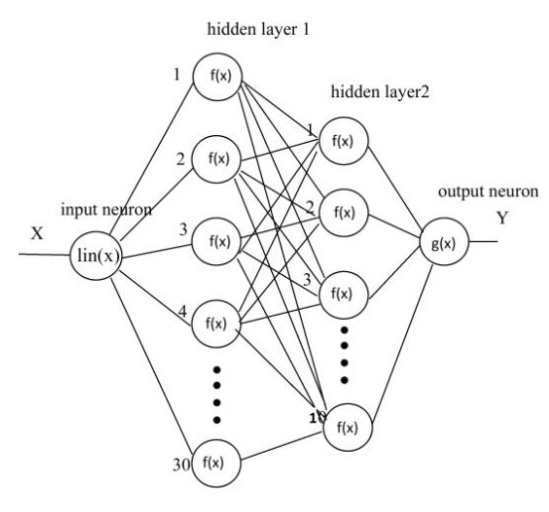
\includegraphics[width=8cm]{net.png}
\centering
\caption{Neural Network Structure}\label{net_img}
\end{figure}
\subsubsection{RBF Neural Network}
Here we use Gaussian function as the radial basis function, shown in equation 5. It can also be interpreted as a rather simple single-layer type of artificial neural network called a radial basis function network, with the radial basis functions taking on the role of the activation functions of the network. 
\begin{equation} \label{eq:3}
\Phi(x) =   {e} ^ {\frac{- {||x-W||} ^ {2}}{{\sigma} ^ {2}}}
\end{equation}\\
\\Where,\\
$\sigma^2$ is variance,\\
x is input, $\Phi(x)$ is output of neuron\\
W is the mean of the sigmoid function or weight of neuron\\
\subsubsection{Extreme learning Machine}
ELM is one step training algorithm, it uses least squares method to estimate the best fit for the weights of the neural network. \\
Here output layer weights are computed, where the hidden layer weights are assigned to the random value. The hidden layer output matrix is assigned as H, then 
\begin{equation} \label{eq:3}
H=XW_{hidden}^T+b_{hidden}
\end{equation}
\begin{equation} \label{eq:4}
W_{out}^T=H^+(y-b_{out})
\end{equation}
\\Where,\\
y is the target data,\\
$H^+$ is the pseudo inverse of H,\\
$b_{hidden}$ is the hidden layer bias vector,\\
$b_{out}$ is output layer bias vector.\\
\subsubsection{Signal conditioning}
The frequency output of the 555 timer varies with the input capacitance in accordance with ().\\
\begin{equation}\label{eq:3}
f=\frac{1}{ln (2)C(R_1+2R_2)}
\end{equation}
Where, \\
f is the frequency output and R1=1MΩ, R2=100KΩ
\begin{figure}[h]
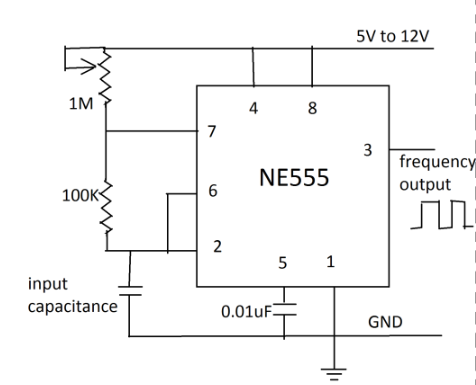
\includegraphics[width=8cm]{ctof.png}
\centering
\caption{capacitance to frequency circuit diagram}\label{ctof_img}
\end{figure}
\\The high time and the low time in each pulse is given by (8) and (9) respectively.\\
\begin{equation} \label{eq:4}
t_{high}= ln(2)C(R_1+R_2)                    
\end{equation}
\begin{equation} \label{eq:5}
t_{low}= ln(2)CR_2                          
\end{equation}
The frequency to voltage converter uses LM331 ic as shown in figure 2. $R_3$ resistance value depends on the supply voltage as shown in equation 9. The output voltage is obtained as shown in equation 10.\\

\begin{equation} \label{eq:6}
 R3= \frac{V_s-2}{2}1000\ \ \Omega           
 \end{equation}               
\begin{equation} \label{eq:4}
V_{out} = 2.09\frac{R_4}{R_5+R_6}R_1C_1VF_{in}  
\end{equation}            
\begin{figure}[h]
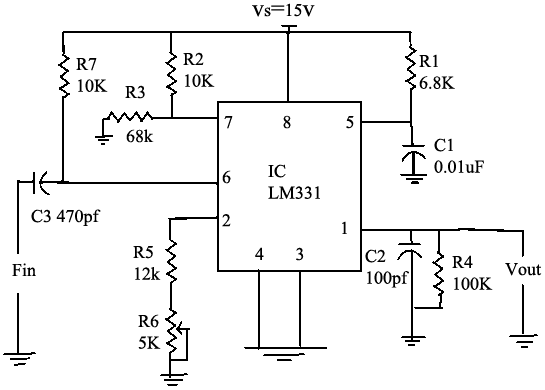
\includegraphics[width=8cm]{ftov.png}
\centering
\caption{frequency to voltage circuit diagram}\label{ftov_img}
\end{figure}
\subsection{Implementation}
ATMega328 microcontroller is used to implement the neural network where the input voltage is taken and their respective outputs are obtained and is displayed. Fig.3 shows the systematic flow. The input, which is level when changes, the capacitance of the cylindrical capacitive sensor changes results in change in frequency output of the capacitance to frequency converter. This frequency output is fed into f/v converter circuit, results a voltage output, this is given as input to ATMega328 microcontroller where the algorithm gives the final level as the output with the compensated non-linearity. \\
\begin{figure}[h]
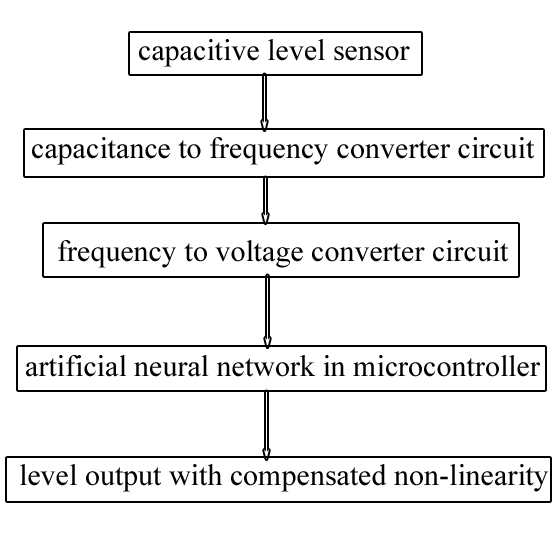
\includegraphics[width=8cm]{blockdiagram.png}
\centering
\caption{Block Diagram}\label{block_diagram_img}
\end{figure}
\begin{figure}[h]
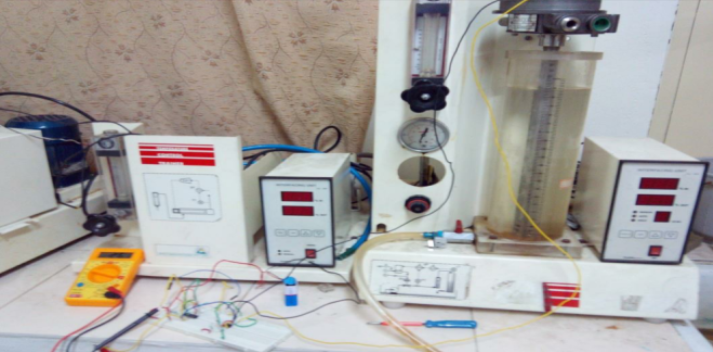
\includegraphics[width=8cm]{setup.png}
\centering
\caption{Experimental Setup}\label{setup_img}
\end{figure}

\subsection{Results}
\begin{center}
  \begin{tabular}{ | l | c  | r |}
    \hline
    Method & Accuracy  & Function used\\ \hline
    Back Propagation (Feed  & 99\% & tansig \\ 
    forward Single layer ANN)&   &         \\ \hline
    ELM(Feed forward&98\% & sig \\ 
     Single layer ANN)&& \\ \hline
    RBF(Feed forward&100\%& gaussian\\  
    Single layer ANN)&& \\
    \hline
  \end{tabular}
%%PLOTS




\end{center}
% An example of a floating figure using the graphicx package.
% Note that \label must occur AFTER (or within) \caption.
% For figures, \caption should occur after the \includegraphics.
% Note that IEEEtran v1.7 and later has special internal code that
% is designed to preserve the operation of \label within \caption
% even when the captionsoff option is in effect. However, because
% of issues like this, it may be the safest practice to put all your
% \label just after \caption rather than within \caption{}.
%
% Reminder: the "draftcls" or "draftclsnofoot", not "draft", class
% option should be used if it is desired that the figures are to be
% displayed while in draft mode.
%
%\begin{figure}[!t]
%\centering
%\includegraphics[width=2.5in]{myfigure}
% where an .eps filename suffix will be assumed under latex, 
% and a .pdf suffix will be assumed for pdflatex; or what has been declared
% via \DeclareGraphicsExtensions.
%\caption{Simulation Results.}
%\label{fig_sim}
%\end{figure}

% Note that IEEE typically puts floats only at the top, even when this
% results in a large percentage of a column being occupied by floats.


% An example of a double column floating figure using two subfigures.
% (The subfig.sty package must be loaded for this to work.)
% The subfigure \label commands are set within each subfloat command,
% and the \label for the overall figure must come after \caption.
% \hfil is used as a separator to get equal spacing.
% Watch out that the combined width of all the subfigures on a 
% line do not exceed the text width or a line break will occur.
%
%\begin{figure*}[!t]
%\centering
%\subfloat[Case I]{\includegraphics[width=2.5in]{box}%
%\label{fig_first_case}}
%\hfil
%\subfloat[Case II]{\includegraphics[width=2.5in]{box}%
%\label{fig_second_case}}
%\caption{Simulation results.}
%\label{fig_sim}
%\end{figure*}
%
% Note that often IEEE papers with subfigures do not employ subfigure
% captions (using the optional argument to \subfloat[]), but instead will
% reference/describe all of them (a), (b), etc., within the main caption.


% An example of a floating table. Note that, for IEEE style tables, the 
% \caption command should come BEFORE the table. Table text will default to
% \footnotesize as IEEE normally uses this smaller font for tables.
% The \label must come after \caption as always.
%
%\begin{table}[!t]
%% increase table row spacing, adjust to taste
%\renewcommand{\arraystretch}{1.3}
% if using array.sty, it might be a good idea to tweak the value of
% \extrarowheight as needed to properly center the text within the cells
%\caption{An Example of a Table}
%\label{table_example}
%\centering
%% Some packages, such as MDW tools, offer better commands for making tables
%% than the plain LaTeX2e tabular which is used here.
%\begin{tabular}{|c||c|}
%\hline
%One & Two\\
%\hline
%Three & Four\\
%\hline
%\end{tabular}
%\end{table}


% Note that IEEE does not put floats in the very first column - or typically
% anywhere on the first page for that matter. Also, in-text middle ("here")
% positioning is not used. Most IEEE journals/conferences use top floats
% exclusively. Note that, LaTeX2e, unlike IEEE journals/conferences, places
% footnotes above bottom floats. This can be corrected via the \fnbelowfloat
% command of the stfloats package.



\section{Conclusion}
All the single layer feed forward neural network, were on the same idea of support vector regression where the 
inputs are mapped to higher dimensions using kernals which we choose in the hidden layer, where classification or regression can be done easily using linear interpreters. \\
Here the response of the capacitive sensor is almost linear but with very small deviations. Where this noise is best interpolated using the gaussian kernal compared to others.\\



% conference papers do not normally have an appendix


% use section* for acknowledgement
\section*{Acknowledgment}


The authors would like to thank...





% trigger a \newpage just before the given reference
% number - used to balance the columns on the last page
% adjust value as needed - may need to be readjusted if
% the document is modified later
%\IEEEtriggeratref{8}
% The "triggered" command can be changed if desired:
%\IEEEtriggercmd{\enlargethispage{-5in}}

% references section

% can use a bibliography generated by BibTeX as a .bbl file
% BibTeX documentation can be easily obtained at:
% http://www.ctan.org/tex-archive/biblio/bibtex/contrib/doc/
% The IEEEtran BibTeX style support page is at:
% http://www.michaelshell.org/tex/ieeetran/bibtex/
%\bibliographystyle{IEEEtran}
% argument is your BibTeX string definitions and bibliography database(s)
%\bibliography{IEEEabrv,../bib/paper}
%
% <OR> manually copy in the resultant .bbl file
% set second argument of \begin to the number of references
% (used to reserve space for the reference number labels box)
\begin{thebibliography}{1}

\bibitem{}
Dempsey, G. L., et al. emph{Control sensor linearization using artificial neural networks.}\hskip 1em plus
  0.5em minus 0.4em\relax Analog Integrated Circuits and Signal Processing 13.3 (1997): 321-332.
\bibitem{}
Patra, Jagdish Chandra, Alex C. Kot, and Ganapati Panda. \emph{An intelligent pressure sensor using neural networks.} \hskip 1em plus
  0.5em minus 0.4em\relax Instrumentation and Measurement, IEEE Transactions on 49.4 (2000): 829-834.
\bibitem{}
Ji, Tao, Qingle Pang, and Xinyun Liu. \emph{An Intelligent Pressure Sensor Using Rough Set Neural Networks.}\hskip 1em plus
  0.5em minus 0.4em\relax Information Acquisition, 2006 IEEE International Conference on. IEEE, 2006. 
\bibitem{}
Medrano-Marqués, Nicolás J., and Bonifacio Martin-del-Brio. \emph{Sensor linearization with neural networks.}\hskip 1em plus
  0.5em minus 0.4em\relax Industrial Electronics, IEEE Transactions on 48.6 (2001): 1288-1290.
\bibitem{}
Khosravi, Mahdi, and Amir Abolfazl Suratgar. \emph{A model of optical micro electro mechanical pressure sensor using artificial neural networks.}\hskip 1em plus
  0.5em minus 0.4em\relax Electrical Engineering (ICEE), 2011 19th Iranian Conference on. IEEE, 2011.
\bibitem{}
 Khosravi, Mahdi, and Amir Abolfazl Suratgar. \emph{A model of optical micro electro mechanical pressure sensor using artificial neural networks.}\hskip 1em plus
  0.5em minus 0.4em\relax Electrical Engineering (ICEE), 2011 19th Iranian Conference on. IEEE, 2011.

\end{thebibliography}




% that's all folks
\end{document}


